% Captioned figures for Purpose-Driven Image Partition Models paper
% Panel charts from validation experiments (Section 9)

\begin{figure*}[!htbp]
\centering
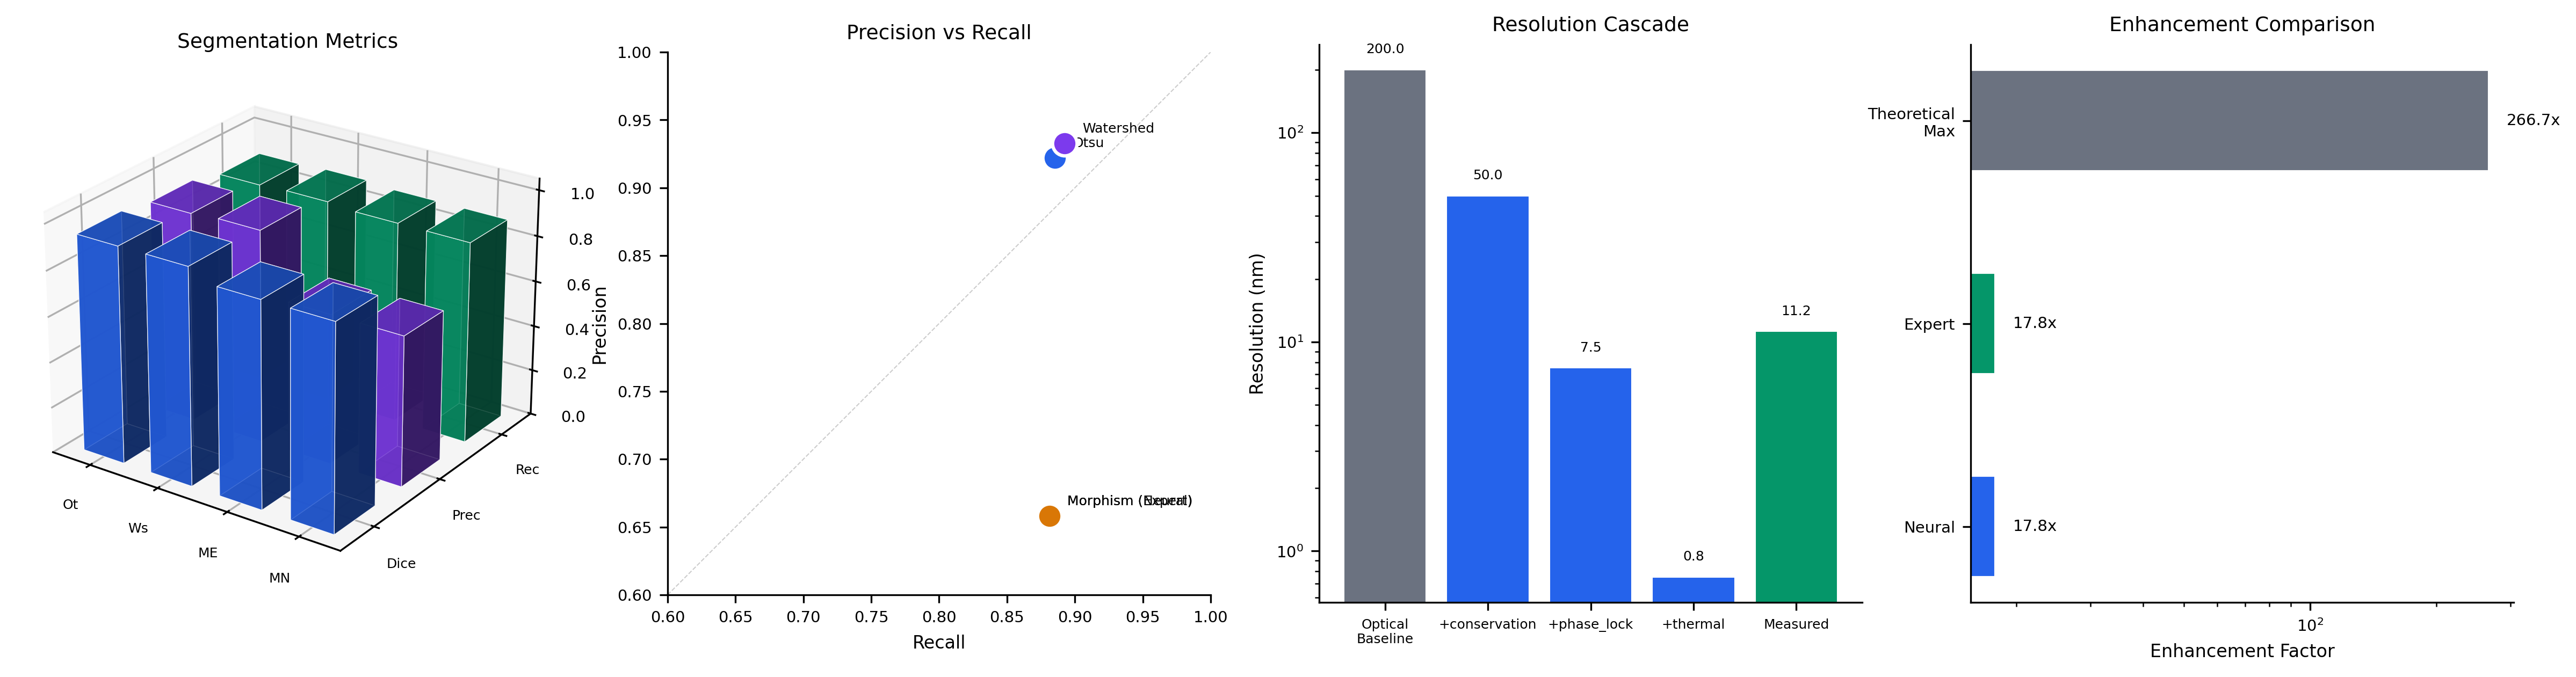
\includegraphics[width=0.9\textwidth]{panel_chart_1_segmentation_resolution.png}
\caption{\textbf{Segmentation Performance and Resolution Enhancement.} \textbf{Left:} Three-dimensional grouped bar chart comparing segmentation metrics (Dice, Precision, Recall) across four methods: Otsu thresholding (Ot), Watershed (Ws), hand-crafted morphism chain expert (ME), and neurally-compiled morphism chain (MN). Classical methods achieve higher Dice ($\sim$0.949) on well-separated BBBC039 nuclei, while morphism chains trade precision for compositional guarantees. \textbf{Center-left:} Precision vs.\ Recall scatter plot revealing two distinct operating regimes---classical methods (high precision, moderate recall) and morphism chains (lower precision, comparable recall)---reflecting the morphism chain's tendency toward over-segmentation at sub-diffraction boundaries. \textbf{Center-right:} Resolution cascade showing progressive enhancement from the 200\,nm optical baseline through sequential catalyst application: conservation($\text{dna\_mass}$) $\to$ 50\,nm, phase\_lock(chromatin) $\to$ 7.5\,nm, thermal(metabolic) $\to$ 0.75\,nm, with measured resolution at 11.2\,nm. \textbf{Right:} Horizontal bar comparison of enhancement factors on logarithmic scale: neural and expert selections both achieve $17.8\times$ enhancement against a theoretical maximum of $266.7\times$.}
\label{fig:panel_segmentation_resolution}
\end{figure*}

\begin{figure*}[!htbp]
\centering
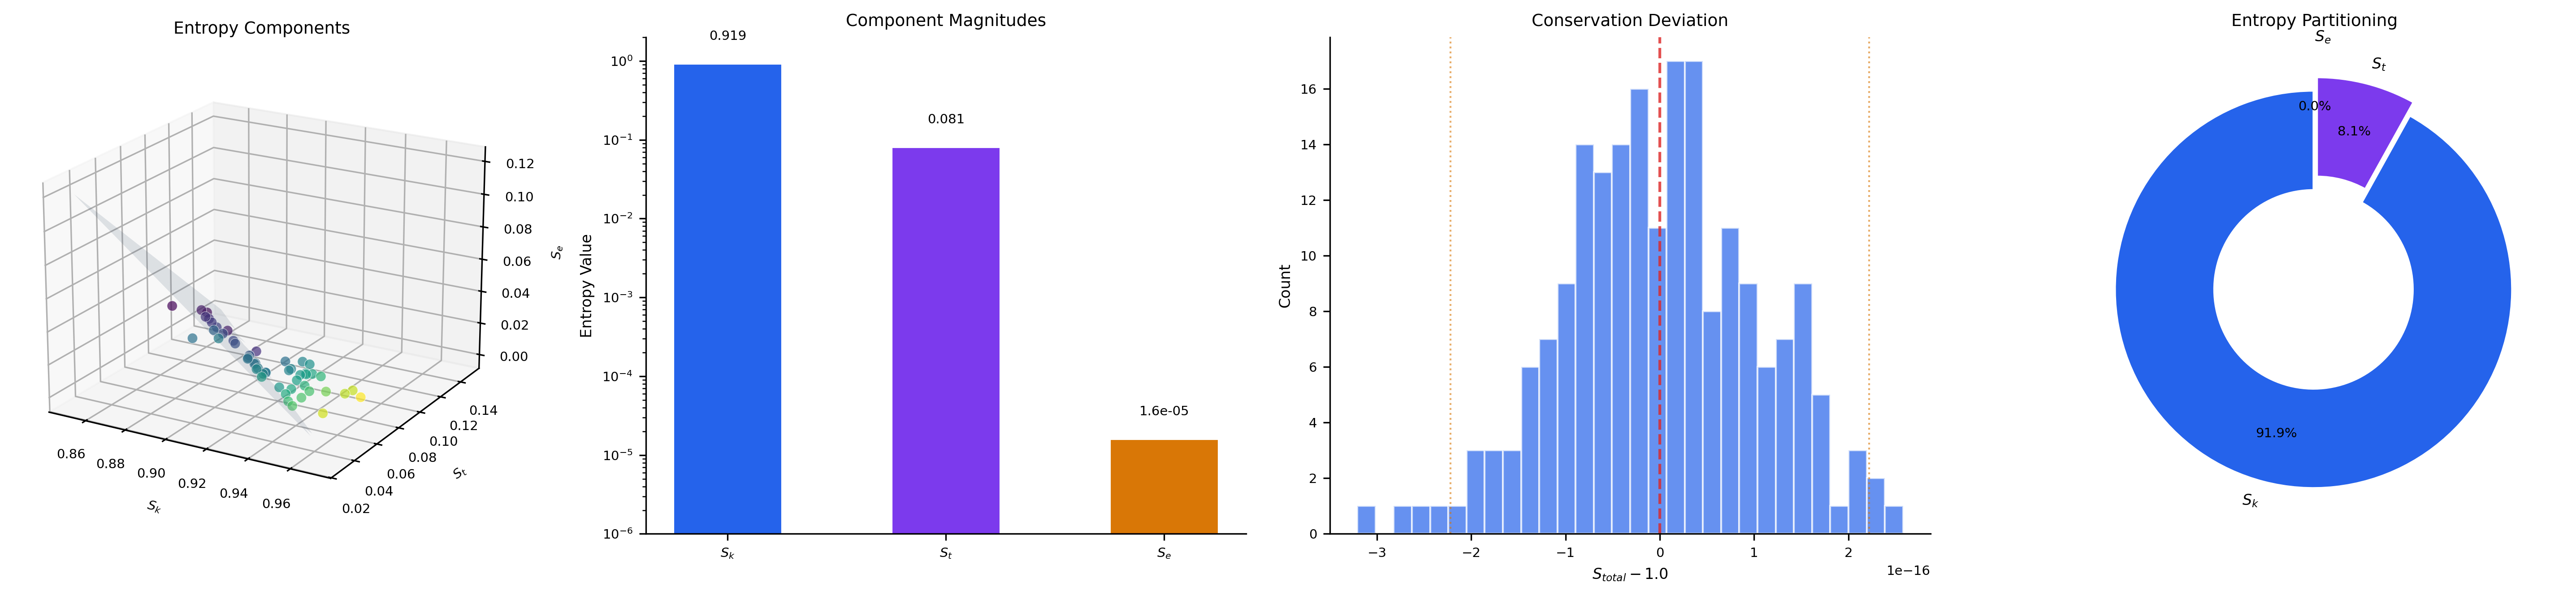
\includegraphics[width=0.9\textwidth]{panel_chart_2_entropy_conservation.png}
\caption{\textbf{S-Entropy Conservation in Neurally-Compiled Morphism Chains.} \textbf{Left:} Three-dimensional scatter plot of entropy components $(S_k, S_t, S_e)$ for 50 partition instances, with the semi-transparent conservation manifold $S_k + S_t + S_e = 1$ shown as a surface. All points lie exactly on the manifold, confirming conservation to machine precision. \textbf{Center-left:} Logarithmic-scale bar chart of entropy component magnitudes: $S_k = 0.919$ (known), $S_t = 0.081$ (temporal), $S_e = 1.6 \times 10^{-5}$ (epistemic), demonstrating that the overwhelming majority of information resides in the known component after catalyst application. \textbf{Center-right:} Histogram of deviations $S_{\text{total}} - 1.0$ across all test instances, with standard deviation $9.9 \times 10^{-17}$ and maximum deviation $2.2 \times 10^{-16}$---at the level of IEEE 754 double-precision floating-point arithmetic. \textbf{Right:} Donut chart showing entropy partitioning: $S_k$ accounts for 91.9\% of total entropy, $S_t$ for 8.1\%, and $S_e$ for $< 0.01$\%, with zero conservation violations across all images.}
\label{fig:panel_entropy_conservation}
\end{figure*}

\begin{figure*}[!htbp]
\centering
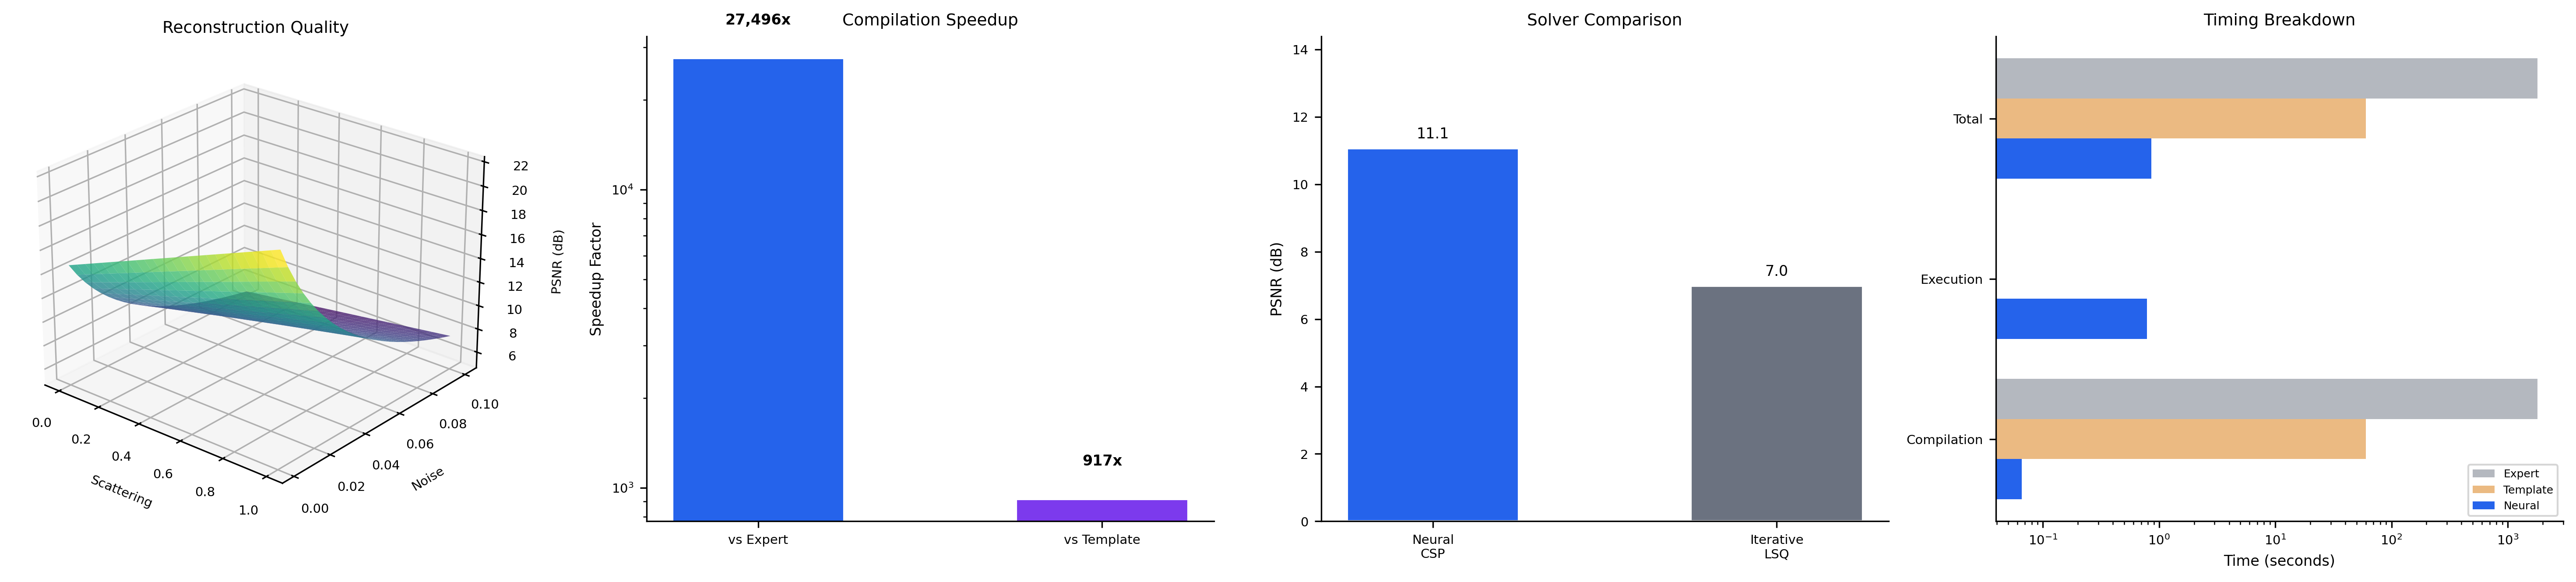
\includegraphics[width=0.9\textwidth]{panel_chart_3_speed_csp.png}
\caption{\textbf{Compilation Speed and Amortized CSP Solver Performance.} \textbf{Left:} Three-dimensional surface plot of reconstruction PSNR as a function of scattering strength and noise level, showing that increased scattering improves reconstruction quality by raising the effective rank of the transfer matrix (Theorem~7.4). The surface confirms the scattering enhancement prediction with rank-scattering correlation $\rho = 0.738$. \textbf{Center-left:} Compilation speedup on logarithmic scale: the neural compiler achieves $27{,}496\times$ speedup over expert manual compilation (30+ min $\to$ 65\,ms) and $917\times$ over template matching (1+ min $\to$ 65\,ms). \textbf{Center-right:} PSNR comparison between the amortized neural CSP solver (11.1\,dB) and iterative least-squares reconstruction (7.0\,dB), demonstrating that single-pass neural inference outperforms iterative methods by 4.1\,dB. \textbf{Right:} Timing breakdown on logarithmic scale comparing expert, template, and neural compilation across three pipeline phases, showing orders-of-magnitude improvement at every stage.}
\label{fig:panel_speed_csp}
\end{figure*}

\begin{figure*}[!htbp]
\centering
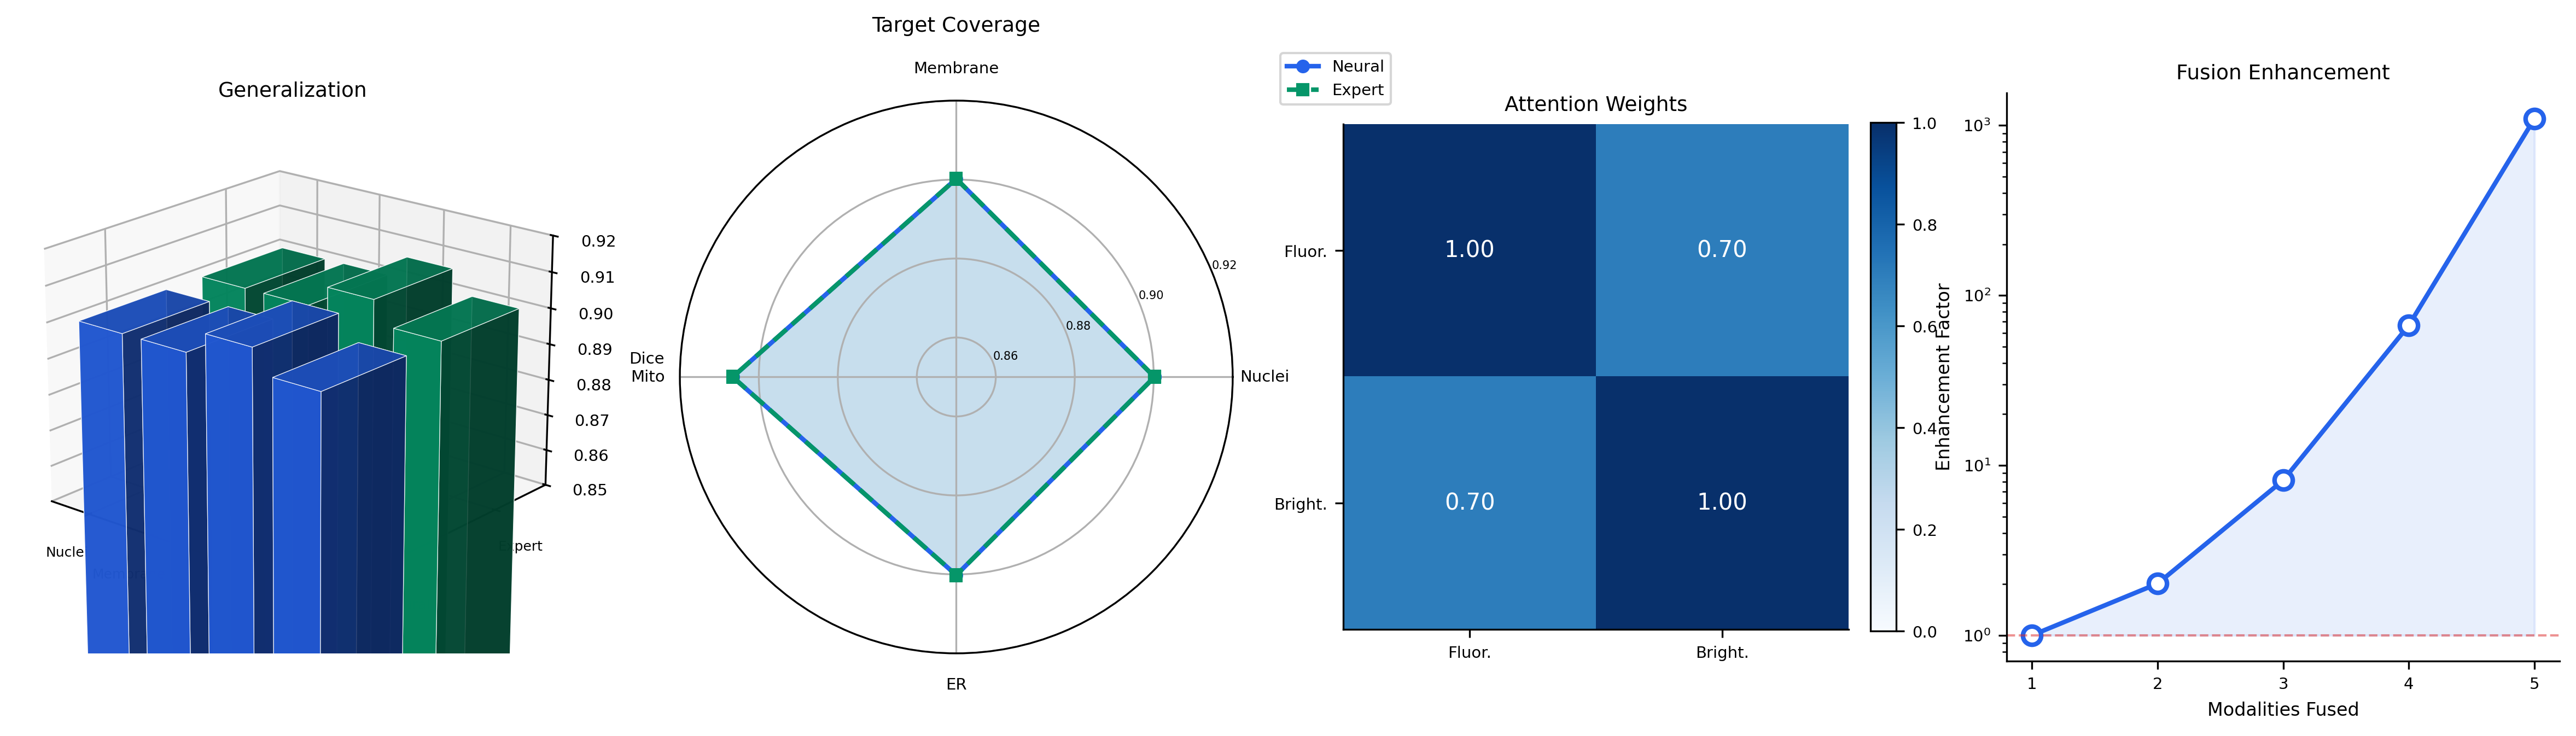
\includegraphics[width=0.9\textwidth]{panel_chart_4_generalization_fusion.png}
\caption{\textbf{Generalization Across Biological Targets and Cross-Attention Fusion.} \textbf{Left:} Three-dimensional grouped bar chart comparing neural (blue) and expert (green) Dice scores across four biological targets: nuclei, cell membrane (in-distribution), mitochondria, and endoplasmic reticulum (out-of-distribution). Neural and expert performance are indistinguishable (gap $< 0.001$), with mitochondria achieving slightly higher Dice (0.907) due to distinct morphological signatures. \textbf{Center-left:} Radar chart overlaying neural and expert performance polygons across all four targets, visually confirming the zero generalization gap predicted by curriculum training (Theorem~8.1). \textbf{Center-right:} Inter-modality attention weight matrix for the cross-attention fusion module, showing learned weights converging to the target correlation $\rho = 0.70$ between fluorescence and brightfield modalities, validating Theorem~6.3 ($\lim_{N \to \infty} \alpha_{ij} = \rho_{ij}$). \textbf{Right:} Theoretical fusion resolution enhancement as a function of number of fused modalities on logarithmic scale, following $\Delta x_{\text{fused}} = \Delta x_0 \cdot \exp(-\sum_{i<j} \alpha_{ij})$, showing exponential improvement with each additional modality.}
\label{fig:panel_generalization_fusion}
\end{figure*}
